\documentclass[paper=a4, fontsize=11pt]{scrartcl}

\usepackage{fancyhdr}
\pagestyle{fancyplain}
\setlength{\headheight}{25pt}
\renewcommand{\headrulewidth}{0pt}
\renewcommand{\footrulewidth}{0pt}
\usepackage{graphicx}
\usepackage{epigraph}
\usepackage{amsmath,amssymb,amsfonts }
\usepackage{lastpage}
\usepackage{algorithm}
\usepackage{algpseudocode}


\newcommand{\Abf}{\ensuremath{\mathbf{A}}}
\newcommand{\bbf}{\ensuremath{\mathbf{b}}}
\newcommand{\cbf}{\ensuremath{\mathbf{c}}}
\newcommand{\abf}{\ensuremath{\mathbf{a}}}
\newcommand{\xbf}{\ensuremath{\mathbf{x}}}
\newcommand{\ybf}{\ensuremath{\mathbf{y}}}
\newcommand{\Rbb}{\ensuremath{\mathbb{R}}}
\newcommand{\Rbf}{\ensuremath{\mathbf{R}}}
\newcommand{\fo}{\ensuremath{f_0}}
\newcommand{\fii}{\ensuremath{f_i}}
\newcommand{\transpose}[1]{#1^\mathsf{T}}
\newcommand{\norm}[1]{\ensuremath{\lVert{#1}\rVert}}


\newtheorem{definition}{Definition}[section]
\newtheorem{theorem}{Theorem}[section]
\newtheorem{lemma}[theorem]{Lemma}
\newtheorem{proposition}[theorem]{Proposition}
\newtheorem{corollary}[theorem]{Corollary}
\newtheorem{observation}[theorem]{Observation}

\newenvironment{proof}[1][Proof]{\begin{trivlist}
\item[\hskip \labelsep {\bfseries #1}]}{\end{trivlist}}
%\newenvironment{definition}[1][Definition]{\begin{trivlist}
%\item[\hskip \labelsep {\bfseries #1}]}{\end{trivlist}}
\newenvironment{example}[1][Example]{\begin{trivlist}
\item[\hskip \labelsep {\bfseries #1}]}{\end{trivlist}}
\newenvironment{remark}[1][Remark]{\begin{trivlist}
\item[\hskip \labelsep {\bfseries #1}]}{\end{trivlist}}

\newcommand{\qed}{\nobreak \ifvmode \relax \else
      \ifdim\lastskip<1.5em \hskip-\lastskip
      \hskip1.5em plus0em minus0.5em \fi \nobreak
      \vrule height0.75em width0.5em depth0.25em\fi}


\newcommand{\lecture}{Homework \#2 Report} %lecture number and date goes here
\newcommand{\lecturedate}{Due: April 11, 2016} %lecture date goeshere
\newcommand{\scribe}{Michael Lam} %student name goes here

\fancyhead[L]{\small Spring 2016}
\fancyhead[R]{\small \lecture}
%\fancyfoot[L]{\small CS 533: Intelligent Agents and Decision Making}
%\fancyfoot[C]{}
\fancyfoot[C]{\thepage\ of \pageref{LastPage}}


\begin{document}


\newcommand{\horrule}[1]{\rule{\linewidth}{#1}} % Create horizontal rule command with 1 argument of height

\title{	
\normalfont \normalsize
\vspace{-30pt}
\textsc{CS 533: Intelligent Agents and Decision Making} \\ [10pt]
\horrule{0.5pt} \\[0.4cm] % Thin top horizontal rule
\LARGE \lecture\\ % The assignment title
\vspace{5pt}
\normalsize \scribe\\
\lecturedate\\
\horrule{2pt} \\[0.5cm] % Thick bottom horizontal rule
}


\date{} % Today's date or a custom date

\maketitle
\vspace{-100pt}
%\epigraph{''Every problem is an optimization problem in disguise.''}{--Anonymous}

\begin{abstract}
This assignment implements finite horizon value iteration and tests the algorithm on some MDPs.
\end{abstract}

\section{Part I}

Run the code as follows:

\begin{verbatim}
python setup.py
source venv/bin/activate
python main.py
deactivate
\end{verbatim}

The setup script creates a Python virtual environment and main.py runs the implemented finite hroizon value iteration algorithm on several MDPs. The setup script is not necessary if numpy is already installed on the system.

\section{Part II}

\subsection{Design}

We design our own MDP for testing purposes as follows. The overview is provided in figure \ref{fig:overview} and the implementation is provided in MDP\_custom.txt. Our MDP has 20 states ($\{ 0, 1, 2, \ldots, 19 \}$). It is a ``cycle'' MDP, where the transition functions for state $i$ only allow the state to go to state $i-1$ or $i+1$ (with wrap-around when in state $0$ or $19$). There are two actions ($\{ 0, 1 \}$). In state $i$, action $0$ has a $0.75$ probability of going to state $i+1$ and $0.25$ probability fo going to state $i-1$. Whereas for action $1$, the probabilities are flipped: in state $i$, the probability of going to state $i+1$ is $0.25$ and the probability of going to state $i-1$ is $0.75$. Intuitively, action $0$ has a greater chance of going to state $i+1$ and action $1$ has a greater chance of going to state $i-1$. Our reward function is as follows: state $19$ has a reward of $1$ and the rest of the states has a reward of $0$.

Intuitively, we can see what the optimal policies are when in certain states with certain time steps to go. We expect to select actions that get the state closer to state $19$.

\begin{figure}
\centering
  	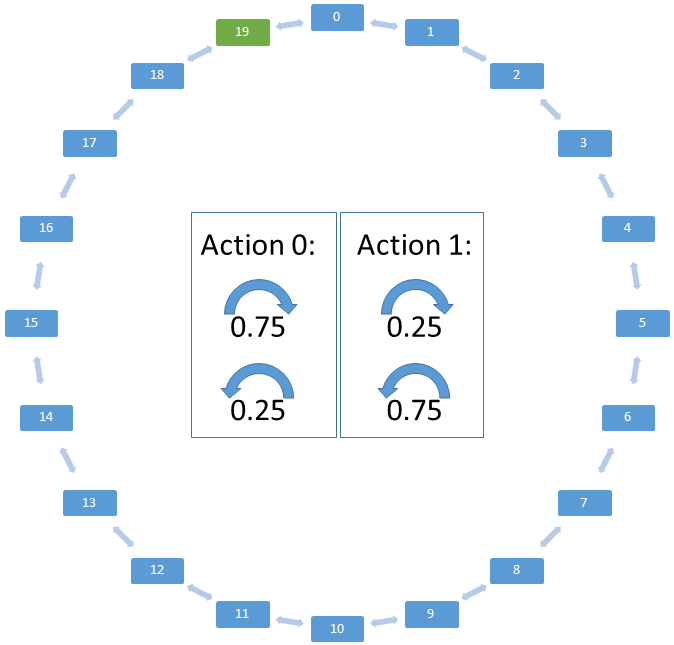
\includegraphics[width=1\linewidth]{assignment2_mdp_figure.png}
\caption{Part II MDP overview. There are $20$ states. State $19$ has reward $1$ and other states have reward $0$. There are two actions: action $0$ has greater probability of going ``clockwise'' and action $1$ has greater probability of going ``counterclockwise.''}
\label{fig:overview}
\end{figure}

\subsection{Results}

For the results below, we will provide the value functions and policies for the MDP. These will be $n \times H$ matrices where rows are the states. For the value functions, column $i$ is the value function with $i$ steps-to-go. For the policies, column $i$ is the policy (i.e. best action) for $i$ steps-to-go.

Below are the value functions for the MDP for horizon $10$. We will show for horizons $1$ and $10$. Note that horizon $1$ is already included in horizon $10$ in the second to last column.

\begin{verbatim}
3.4890  2.8160  2.8160  2.1387  2.1387  1.4531  1.4531  0.7500  0.7500  0.0000
2.5079  2.5079  1.8479  1.8479  1.1953  1.1953  0.5625  0.5625  0.0000  0.0000
2.2177  1.5837  1.5837  0.9756  0.9756  0.4219  0.4219  0.0000  0.0000  0.0000
1.3472  1.3472  0.7910  0.7910  0.3164  0.3164  0.0000  0.0000  0.0000  0.0000
1.1383  0.6378  0.6378  0.2373  0.2373  0.0000  0.0000  0.0000  0.0000  0.0000
0.5117  0.5117  0.1780  0.1780  0.0000  0.0000  0.0000  0.0000  0.0000  0.0000
0.4088  0.1335  0.1335  0.0000  0.0000  0.0000  0.0000  0.0000  0.0000  0.0000
0.1001  0.1001  0.0000  0.0000  0.0000  0.0000  0.0000  0.0000  0.0000  0.0000
0.0751  0.0000  0.0000  0.0000  0.0000  0.0000  0.0000  0.0000  0.0000  0.0000
0.0000  0.0000  0.0000  0.0000  0.0000  0.0000  0.0000  0.0000  0.0000  0.0000
0.0751  0.0000  0.0000  0.0000  0.0000  0.0000  0.0000  0.0000  0.0000  0.0000
0.1001  0.1001  0.0000  0.0000  0.0000  0.0000  0.0000  0.0000  0.0000  0.0000
0.4088  0.1335  0.1335  0.0000  0.0000  0.0000  0.0000  0.0000  0.0000  0.0000
0.5117  0.5117  0.1780  0.1780  0.0000  0.0000  0.0000  0.0000  0.0000  0.0000
1.1383  0.6378  0.6378  0.2373  0.2373  0.0000  0.0000  0.0000  0.0000  0.0000
1.3472  1.3472  0.7910  0.7910  0.3164  0.3164  0.0000  0.0000  0.0000  0.0000
2.2177  1.5837  1.5837  0.9756  0.9756  0.4219  0.4219  0.0000  0.0000  0.0000
2.5079  2.5079  1.8479  1.8479  1.1953  1.1953  0.5625  0.5625  0.0000  0.0000
3.4890  2.8160  2.8160  2.1387  2.1387  1.4531  1.4531  0.7500  0.7500  0.0000
3.8160  3.8160  3.1387  3.1387  2.4531  2.4531  1.7500  1.7500  1.0000  1.0000
\end{verbatim}

Here are the policies for the MDP:

\begin{verbatim}
1       1       1       1       1       1       1       1       1       0
1       1       1       1       1       1       1       1       0       0
1       1       1       1       1       1       1       0       0       0
1       1       1       1       1       1       0       0       0       0
1       1       1       1       1       0       0       0       0       0
1       1       1       1       0       0       0       0       0       0
1       1       1       0       0       0       0       0       0       0
1       1       0       0       0       0       0       0       0       0
1       0       0       0       0       0       0       0       0       0
0       0       0       0       0       0       0       0       0       0
0       0       0       0       0       0       0       0       0       0
0       0       0       0       0       0       0       0       0       0
0       0       0       0       0       0       0       0       0       0
0       0       0       0       0       0       0       0       0       0
0       0       0       0       0       0       0       0       0       0
0       0       0       0       0       0       0       0       0       0
0       0       0       0       0       0       0       0       0       0
0       0       0       0       0       0       0       0       0       0
0       0       0       0       0       0       0       0       0       0
0       0       0       0       0       0       0       0       0       0
\end{verbatim}

\subsection{Analysis}

For horizon $1$, it is easy to see the policy that we expect. If we start in state $0$, then selecting action $1$ will have a greater chance of going to state $19$ to get the reward than action $0$. In fact, the value function is also correct: the expectation is $0.75$ since the reward is $1$ for going to state $19$ with probability $0.75$ and the reward is $0$ for going to state $1$. Similarly if we start in state $18$, then selecting action $0$ will have a greater chance of going to state $19$ than action $1$. Again, the value function also makes sense. If we start in state $19$, then whatever action is taken will not yield a reward since it has to go to state $18$ or $0$. However, it has reward $1$ for being in state $19$ at first, which is reflected in the value function. Finally, all other states have a $0$ expected reward since in one time step it is impossible to reach state $19$.

For horizon $10$, we see that the policies are changed so that taking the optimal actions will advance the current state nearer to the reward state $19$. Given more time horizon, the states that can reach $19$ now yield non-zero values for expected reward and thus the policy is changed as a function of the time horizon. Note that state $9$ still cannot reach state $19$ in $9$ steps, thus the expected reward is still $0$ for it.

\section{Part III}

In this section we provide the value functions and policies for MDPs 1 and 2. These will be $n \times H$ matrices where rows are the states. For the value functions, column $i$ is the value function with $i$ steps-to-go. For the policies, column $i$ is the policy (i.e. best action) for $i$ steps-to-go.

Here are the value functions for MDP1:

\begin{verbatim}
3.0330  3.0000  3.0000  2.0330  2.0000  2.0000  1.0330  1.0000  1.0000  0.0000
2.9998  2.8944  2.0184  1.9998  1.8944  1.0184  0.9998  0.8944  0.0000  0.0000
2.8982  2.7992  2.0126  1.8982  1.7992  1.0126  0.8982  0.7987  0.0074  0.0000
2.9039  2.8944  2.0184  1.9039  1.8944  1.0184  0.9039  0.8944  0.0000  0.0000
4.0000  3.0330  3.0000  3.0000  2.0330  2.0000  2.0000  1.0330  1.0000  1.0000
2.8944  2.6524  1.9998  1.8944  1.6527  0.9998  0.8944  0.6595  0.0000  0.0000
2.9804  2.8783  2.6524  1.9804  1.8784  1.6527  0.9812  0.8806  0.6595  0.0000
2.8958  2.8524  2.0125  1.8958  1.8524  1.0125  0.8960  0.8522  0.0000  0.0000
3.0000  3.0000  2.0330  2.0000  2.0000  1.0330  1.0000  1.0000  0.0330  0.0000
3.0184  2.9039  2.8944  2.0184  1.9039  1.8944  1.0184  0.9039  0.8944  0.0000
\end{verbatim}

Here are the policies for MDP1:

\begin{verbatim}
3       3       3       3       3       3       3       3       3       0
1       3       3       1       3       3       1       3       0       0
1       2       2       1       2       2       1       2       2       0
0       0       0       0       0       0       0       0       0       0
0       0       0       0       0       0       0       0       0       0
2       0       2       2       0       2       2       0       0       0
1       1       1       1       1       1       1       1       1       0
2       2       2       2       2       2       2       2       0       0
1       1       1       1       1       1       1       1       3       0
3       0       3       3       0       3       3       0       3       0
\end{verbatim}

Here are the value functions for MDP2:

\begin{verbatim}
4.0569  4.0000  3.0569  3.0000  2.0569  2.0000  1.0569  1.0000  0.0569  0.0000
3.9952  3.9919  2.9952  2.9919  1.9952  1.9919  0.9950  0.9925  0.0000  0.0000
5.3085  4.6244  4.3081  3.6236  3.3062  2.6193  2.2970  1.5991  1.2527  0.4931
3.9927  3.0419  2.9928  2.0420  1.9929  1.0419  0.9936  0.0665  0.0006  0.0000
4.5715  4.0000  3.5715  3.0000  2.5715  2.0000  1.5715  1.0000  0.5715  0.0000
5.0000  4.0003  4.0000  3.0003  3.0000  2.0003  2.0000  1.0002  1.0000  0.0000
5.0003  5.0000  4.0003  4.0000  3.0003  3.0000  2.0002  2.0000  1.0000  1.0000
3.9648  3.0813  2.9648  2.0813  1.9648  1.0813  0.9657  0.0816  0.0775  0.0000
4.0000  3.5715  3.0000  2.5715  2.0000  1.5715  1.0000  0.5715  0.0112  0.0000
5.0000  4.0003  4.0000  3.0003  3.0000  2.0003  2.0000  1.0000  0.9999  0.0000
\end{verbatim}

Here are the policies for MDP2:

\begin{verbatim}
3       0       3       0       3       0       3       0       3       0
0       0       0       0       0       0       0       0       0       0
0       0       0       0       0       0       0       0       0       0
1       1       1       1       1       1       1       2       1       0
2       1       2       1       2       1       2       1       2       0
2       0       2       0       2       0       2       0       2       0
2       2       2       2       2       2       2       2       0       0
1       1       1       1       1       1       1       1       3       0
0       1       0       1       0       1       0       1       3       0
2       2       2       2       2       2       2       2       2       0
\end{verbatim}

\end{document}